\section{Программное обеспечение IoT}
Программное обеспечение IoT обращается к своим ключевым областям работы в сети и действиям с помощью платформ, embeded-системы
, партнерские системы и промежуточное ПО. Эти основные приложения
отвечает за сбор данных, интеграцию устройств, аналитику в реальном времени, приложения и
расширение процесса в сети IoT. Они используют интеграцию с критически важными бизнес-системами
(например, системы заказов, робототехника, систем планирование и т. д.) при выполнении связанных задач.

\subsection{Сбор информации}
Это программное обеспечение управляет датчиками, измерениями, фильтрацией данных, безопасностью этих данных и
агрегацией данных. ПО использует определенные протоколы, чтобы помочь датчикам подключаться к данным в реальном времени.
Один из вариантов сбора данных в IoT системах визуализирован на рисунке \ref{fig:section5:data_collecting}.

\begin
{figure}[h!]
    \centering
    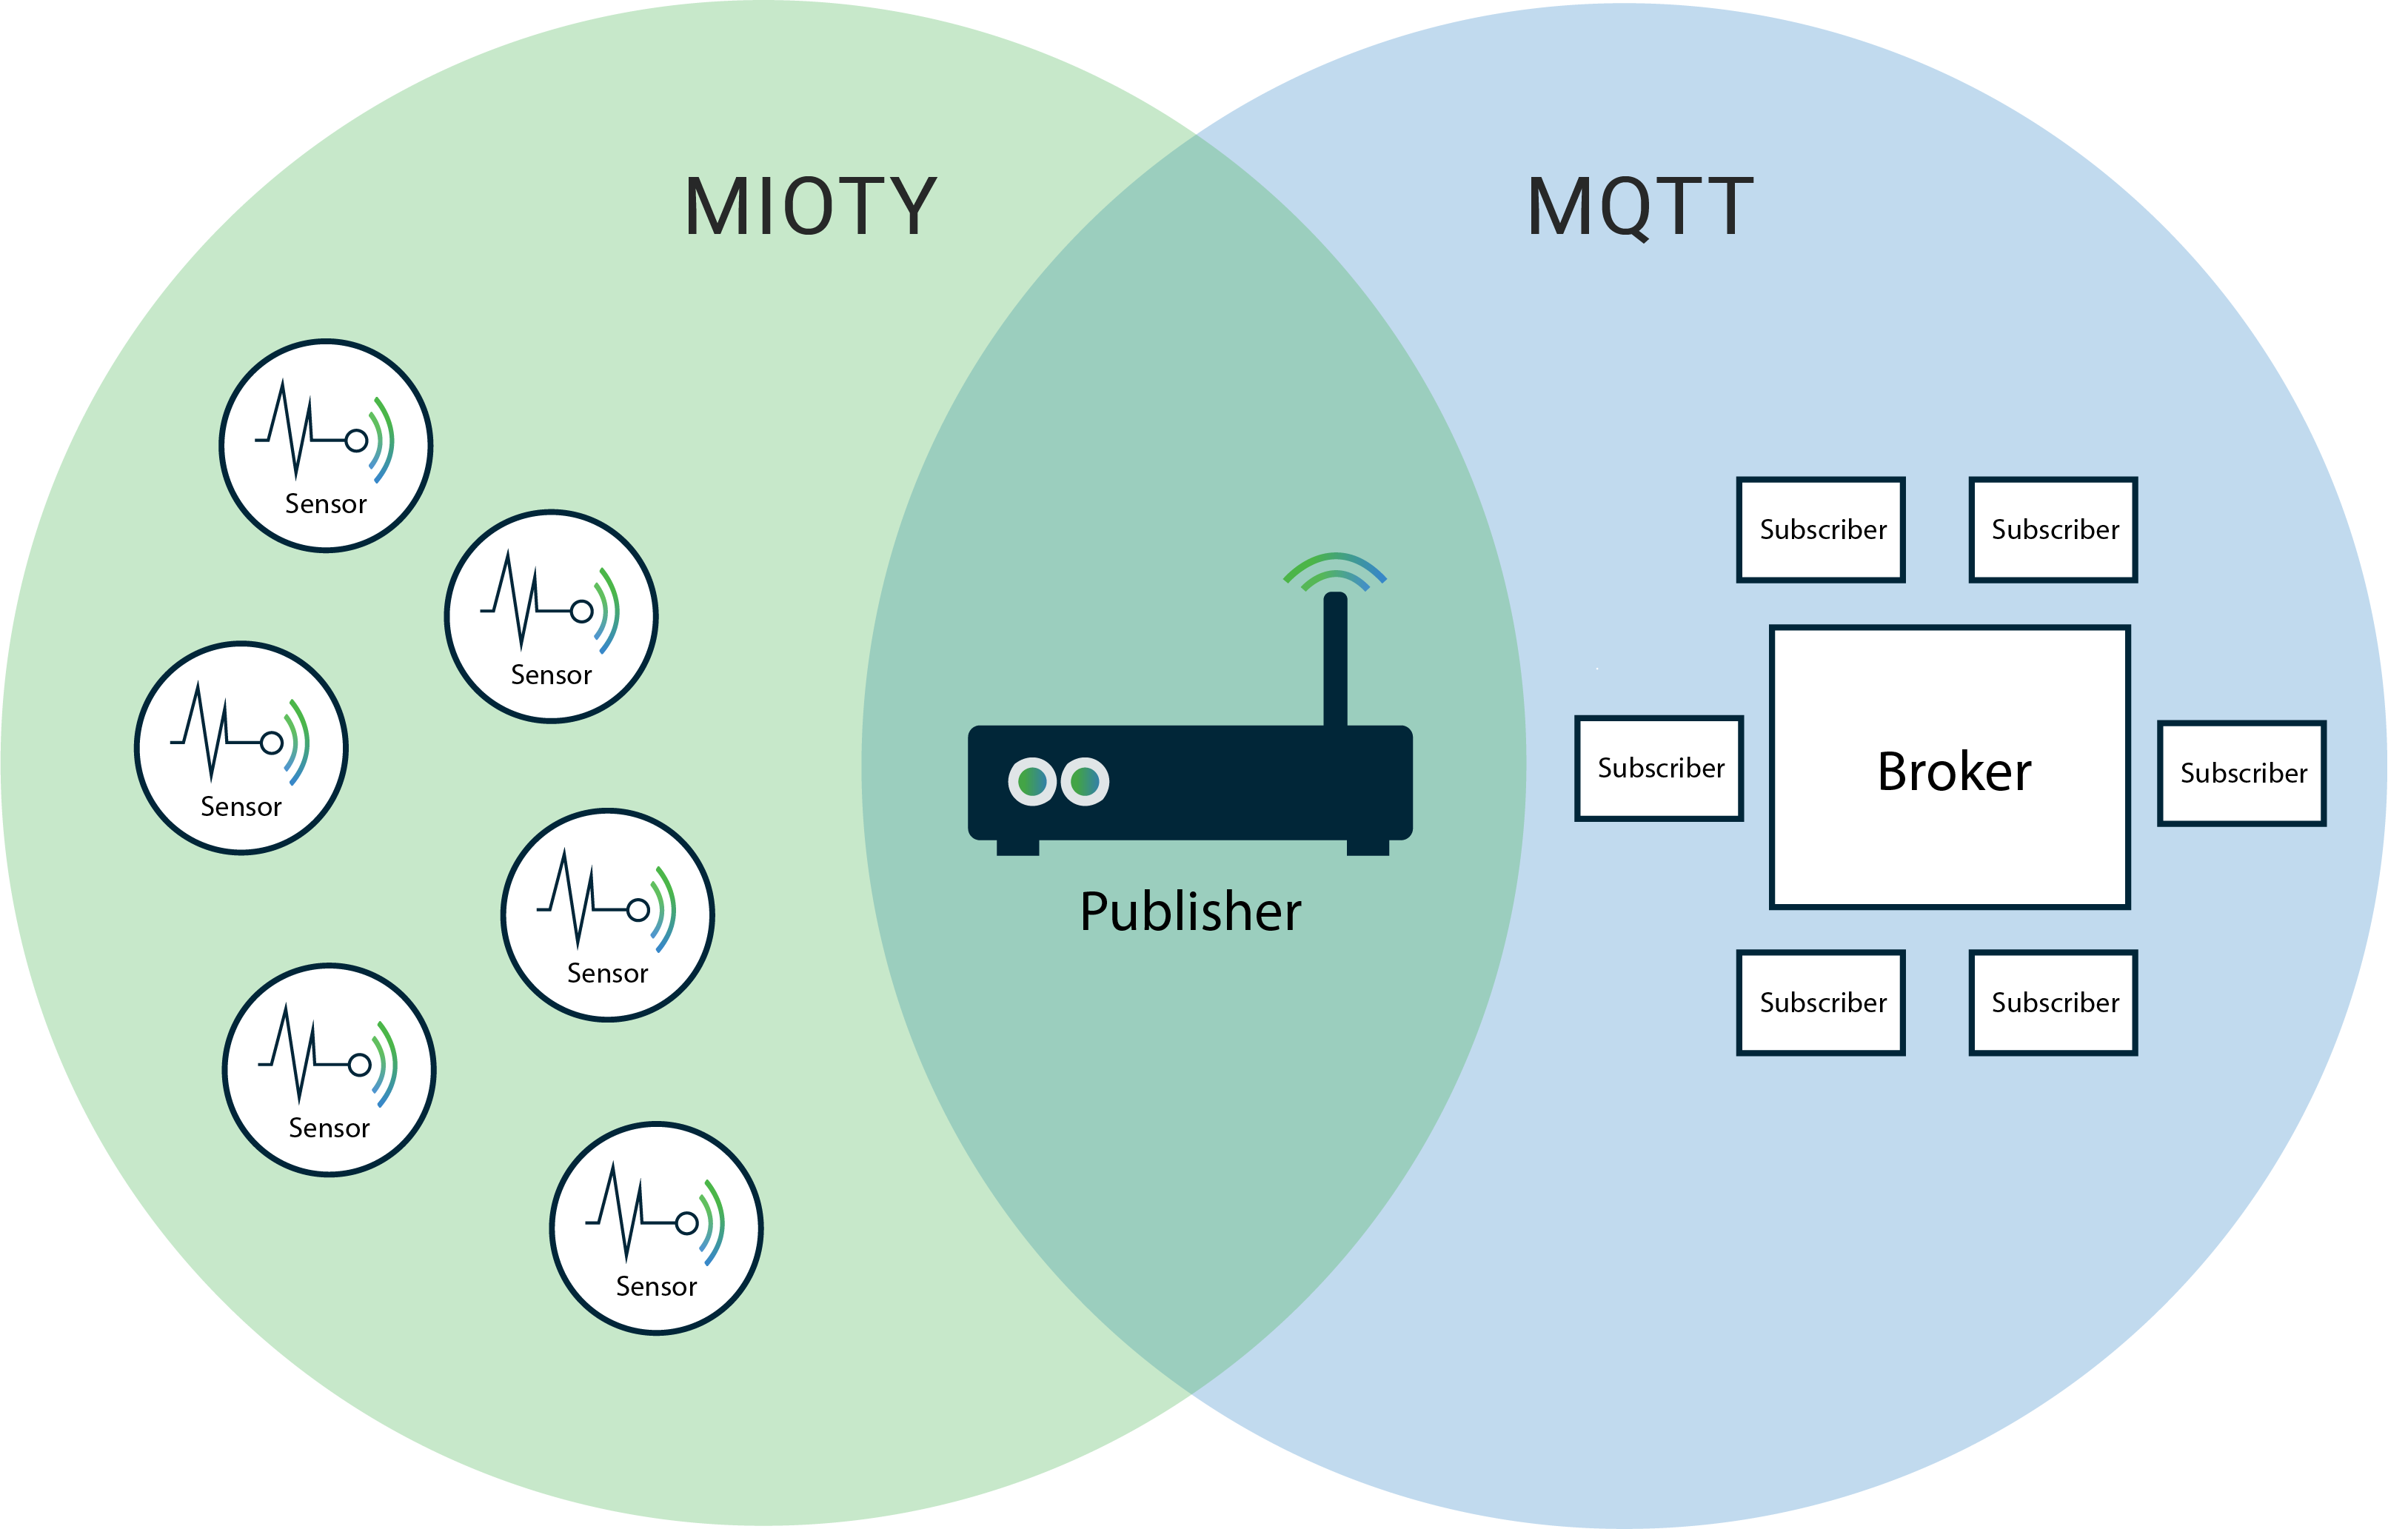
\includegraphics[scale=0.3]{data_collecting.png}
    \caption{Диаграмма сбора данных в системе IoT}
    \label{fig:section5:data_collecting}
\end{figure}

Затем ПО собирает данные с нескольких устройств и распределяет их в
соответствии с конфигурацией. ПО также работает и в обратном порядке, распределяя данные по устройствам в зависимости от их назначения. Система
в конечном итоге передает все собранные данные на центральный сервер.

\subsection{Интеграция устройств}
Программное обеспечение, поддерживающее интеграцию, связывает (зависимые отношения) все системные устройства для создания
тело системы IoT. Это обеспечивает необходимое сотрудничество и стабильное соединение между
устройствами. Эти приложения являются определяющей программной технологией сети IoT, поскольку
без них это не система IoT. Они управляют различными приложениями, протоколами и
ограничения каждого устройства для обеспечения связи.\cite{IoTAzure}

\subsection{Аналитика  в реальном времени}
Эти приложения берут входные данные с различных устройств и преобразуют их в рельаные действия или действия, 
которые пригодны для обнаружения закономерности. На рисунке \ref{fig:section5:realtime} представлен пример аналитики в реальном временени в разрезе системы умного дома.

\begin
{figure}[h!]
    \centering
    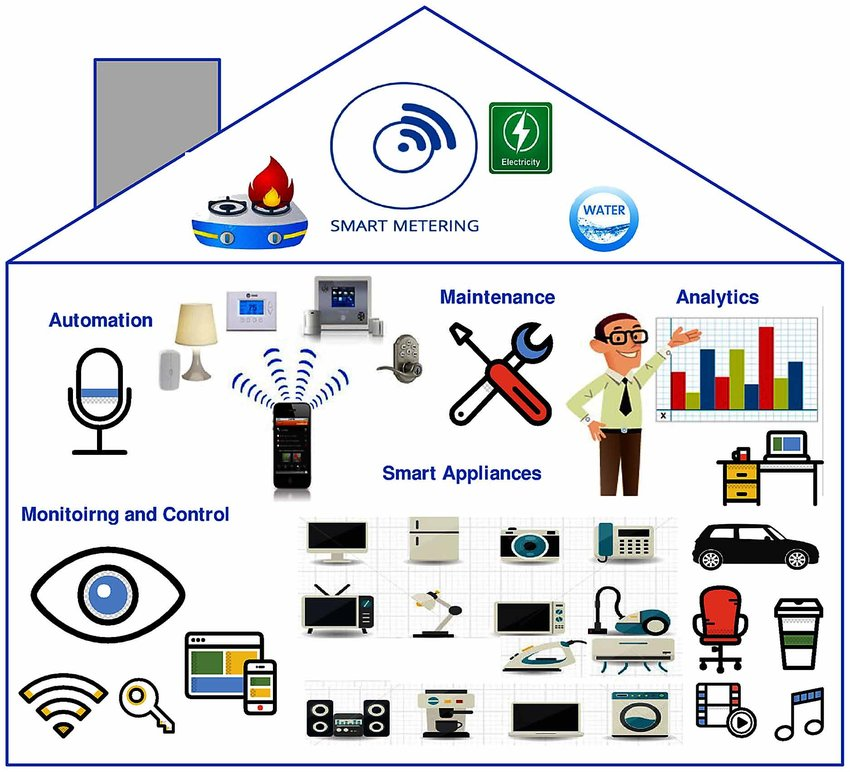
\includegraphics[scale=0.3]{realtime.png}
    \caption{Обработка данных и дальнейшая взаимосвязь между устройствами}
    \label{fig:section5:realtime}
\end{figure}

Они анализируют информацию на основе различных настроек и
установленного заранее для выполнения задач, связанных с автоматизацией, или предоставления данных, требуемых промышленностью.